\chapter{Evaluation}
\label{sec:evaluation}

% Zu jeder Arbeit in unserem Bereich gehört eine Leistungsbewertung. Aus
% diesem Kapitel sollte hervorgehen, welche Methoden angewandt worden,
% die Leistungsfähigkeit zu bewerten und welche Ergebnisse dabei erzielt
% wurden. Wichtig ist es, dem Leser nicht nur ein paar Zahlen
% hinzustellen, sondern auch eine Diskussion der Ergebnisse
% vorzunehmen. Es wird empfohlen zunächst die eigenen Erwartungen
% bezüglich der Ergebnisse zu erläutern und anschließend eventuell
% festgestellte Abweichungen zu erklären.

The following chapter presents the measurement setup and the final benchmarks used for this thesis and the test cases they were used in as well as a discussion of the results.
The implemented load balancer is compared to the Linux EEVDF scheduler and also measured for overhead and scalability in different configurations.

\section{Measurement Setup and Benchmarks}

\paragraph{Hardware.}

The load balancing component is tested on the Intel Core i9-13900K, a processor with 32 hardware threads.
It follows the Intel hybrid architecture mentioned in Section~\ref{sec:amp}, with eight performance cores that have two hardware threads each and 16 efficiency cores housing one hardware thread.
Additionally, this server has access to 128 GB of DDR5 main memory clocked at \SI{3600}{\mega\hertz}.

\paragraph{Operating System Comparison.}
\label{sec:os-comparison}

The implementation is tested against the well-engineered Linux scheduler; that means that the benchmarks used need to behave similarly on both operating systems.
Hence, established benchmarks are used to construct multiple test cases that can be compared across the boundaries of operating systems.
One problem is that operating systems are complex programs that are made up of more than just a scheduler.
Therefore, multiple components have an influence on execution speed next to the scheduler.

\paragraph{Algorithms.}

The strategies tested during the evaluation are the native L4Re microkernel scheduler, the developed load balancer in two versions, and the Linux EEVDF scheduler.
The first developed version does no periodic balancing but statically assigns a new thread the CPU with the lowest current \texttt{vload} and is therefore static as it operates in 100 \si{\ms} monitoring intervals; it will be referred to as STA100 from now on.
The second variant of the load balancer also includes rebalancing as described in Section~\ref{sec:rebalancing}.
Although both versions make use of the CPU performance scaling explained in Section~\ref{sec:cpu-performance}, the second version will be referred to as AMP.
The AMP balancer is also tested with multiple intervals of the monitoring period (10, 20, 50, 100 \si{\ms}); these will be referenced as AMP<N> with N being the duration of the interval.

\section{SPEC CPU Benchmarks}

The SPEC CPU benchmarking suites\footnote{\url{https://www.spec.org/cpu}} are an established framework to benchmark the hardware it is tested on.
SPEC aims to design benchmarks that try to represent real-world workloads.
Therefore, choosing unique instances from their suites to combine them into test cases that represent real-world scenarios is straightforward.
The SPEC CPU benchmarks were regarded for this work because they are well-tested and already used in previous work done in the field by Eppelt~\cite{philipp-thesis}.

\subsection{SPEC CPU 2006}

The SPEC CPU 2006 benchmark suite\footnote{\url{https://www.spec.org/cpu2006}} contains four tests that cover a wide range of use cases.
Namely, \texttt{403.gcc} representing compiler tasks based on integer computation, \texttt{429.mcf} calculating combinatorial optimization through integers, \texttt{462.libquantum} executing quantum physics integer calculations, and \texttt{470.lbm} doing fluid dynamics based on floating-point operations.
Although the suite is retired and therefore could seem outdated, this fact does not pose a problem, as the benchmarking tests the load balancer, its overhead, and decision-making instead of targeting the hardware.
Additionally, the hardware demands of up to one GB per instance allowed for a significant number of instances at once on the given hardware.

\paragraph{Infeasibility.}

In Section~\ref{sec:cpu0-problem}, it was discussed that freeing memory in L4Re is the task of Moe because it needs to unmap all pages.
With every SPEC CPU 2006 instance occupying up to one GB of main memory according to their specification.
When done in 4 KiB pages, this leads to thousands of pages that need to be unmapped when a single instance finishes execution, monopolizing CPU0 in the process.
This alone is suboptimal, but those benchmarks verify their computation by printing information to serial output; every thread was additionally waiting for its \texttt{printf()} calls to be handled as well.
This behavior results in every thread on every CPU waiting for Moe on CPU0 to become available and handle either their memory unmapping or their standard output.
Finally defeating the purpose of having independent processing instances that need to be scheduled because the bottleneck of the system is the handling of serial output and not the efficiency of the load balancing service developed throughout this thesis.

\subsection{SPEC CPU 2017}

The 2017 suite\footnote{\url{https://www.spec.org/cpu2017}} of SPEC CPU provides three out of the four benchmarks chosen from the 2006 suite.
Therefore, the updated versions \texttt{505.mcf\_r} and \texttt{519.lbm\_r} were ported to the L4Re environment.

\paragraph{Infeasibility.}

Unfortunately, a single instance of these benchmarks runs for almost 10 minutes making it unsuitable for multi threaded execution despite the memory unmapping problem. This also makes the latest release of the SPEC CPU 2026 suite infeasible, because it has the same 2 GB memory requirements per thread and is expected to have an even longer runtime than its 2017 predecessor. 

\section{Used Benchmarks}
\label{sec:bench-used}

The aim was still to cover a wide range of real-world workloads, leading to benchmarks being selected that have comparable characteristics to the SPEC CPU 2006 benchmarks.
The four programs being ported to L4Re ended up being CoreMark\footnote{\url{https://github.com/eembc/coremark}}, STREAM\footnote{\url{https://www.cs.virginia.edu/stream/FTP/Code}}, Whetstone\footnote{\url{https://www.netlib.org/benchmark/whetstone.c}}, and tinymembench\footnote{\url{https://github.com/ssvb/tinymembench}}.
CoreMark performs integer computation and function calls, STREAM tests pointer chasing, Whetstone covers floating-point and math operations, and tinymembench measures memory bandwidth and latency.
All these benchmarks were be ported to L4Re and Linux, making them suitable for the scope of this work.
Unfortunately, STREAM and tinymembench suffer from the same problem as the SPEC CPU benchmarks, although their memory usage got reduced below 10 MB.
Leaving only CoreMark and Whetstone for the final validation runs.

\paragraph{Modifications.}

To avoid thread blocking of the benchmark instances, the serial output in the benchmarks is disabled (see Section~\ref{sec:cpu0-problem}).
CoreMark has an \texttt{ITERATIONS} parameter that was set to \texttt{1'000'000}.
Similarly, Whetstone has its \texttt{LOOP} count set to \texttt{100'000} in combination with the iteration value \texttt{II} with \texttt{100}.
Both these modifications ensure that the benchmarks run for a sufficient and similar time.

\section{Test Cases}
\label{sec:test-cases}

\paragraph{Baseline.}

For this test, a benchmark is run single-threaded sequentially until 100 instances are reached.
The scheduler should only need to decide once on which CPU the single instance is to be executed.
The baseline sets an anchor point to compare the results of following test cases.
It also allows for the usage of the native L4Re scheduler, as it will always schedule any thread on CPU0 that does not have a specific CPU set passed along with it.
Further, it helps to expose differences in execution speeds caused by Linux or L4Re, which are not related to the scheduler.
The investigated schedulers are the native L4Re kernel scheduler, STA100, AMP100, and Linux EEVDF.

\paragraph{CPU Scalability.}

This scenario investigates the scalability of schedulers by assigning them the same numbers of CoreMark threads as they have CPUs to distribute them until 100 instances are finished.
The number of parallel threads and CPUs used are 2, 4, and 8.

\begin{figure}
	\centering
	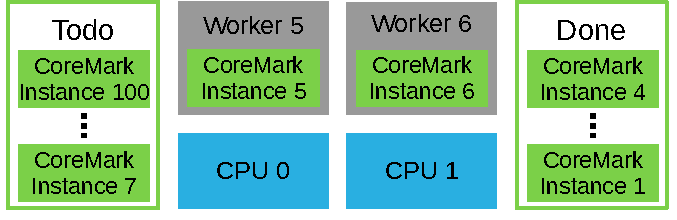
\includegraphics[width=0.7\textwidth]{images/cpu_scaling.pdf}
	\caption{CPU scalability test for two parallel worker threads and two CPUs with 100 CoreMark instances to be computed. Four instances are already done, two are being processed, and 94 need to be spawned and done.}
	\label{fig:cpu-scalability}
\end{figure}


This test represents workloads that can be executed multithreaded.
A common example is the compiler program \texttt{make} used with the additional option of \texttt{-jN}, where N is the number of parallel jobs that are started to finish the compilation.
The investigated schedulers are the static balancer, all four AMP variants, and Linux EEVDF.

\paragraph{Parallel Execution.}

The effect of a well-designed load balancing algorithm shows the most when stressed to the extent of its capabilities.
To mimic this, the parallel execution test contains three cases simulating low, full, and overload by running 8, 16, and 64 instances of each of the CoreMark and Whetstone benchmarks in parallel until 100 instances are finished for each.
To keep the CPU load up consistently at all times, new threads are spawned even when one benchmark reaches its target count until the slower of the two benchmarks finishes its 100 instances.
All three cases test the same schedulers as were already investigated in the CPU scalability scenario.

\paragraph{Monitoring Scalability.}

During the monitoring scalability tests, no benchmarks were used but a custom benchmarking harness for the AMP balancer.
It captures the execution times of the scheduling proxy, commander, and monitors of the AMP balancer with all its four monitoring periods.
Additionally, it tests if the parallel (AMP<N>P) approach to \texttt{vload} updates is superior to the centralized (AMP<N>C) solution argued in Section~\ref{sec:vload-updates}.
All configurations are tracked during the monitoring of 0, 10, 100, 500, 1000, and 2000 idle threads; the spawning parent thread, ITAS, and an additional thread called the pthread manager for a duration of \SI{100}{\second}.
The data points for 0 idle threads are similar to 10 idle threads and are therefore left out for plot readability.
The pthread manager is only spawned whenever the application's main thread spawns at least one additional thread.

\section{Results}

This section presents the results of the benchmarks specified in Section~\ref{sec:bench-used} with their corresponding modifications run in the test cases of Section~\ref{sec:test-cases}.
Further plots of the benchmarks' execution times can be found in Section~\ref{sec:appendix}.

\paragraph{Box Plots.}

As a means of visualizing the 100 single runs of the CoreMark and Whetstone, benchmark box plots were used.
They provide a compact visualization of a data set's distribution by summarizing it through six components. 
The first quartile ($Q_1$) represents the value below which 25\,\% of the data points fall, marking the bottom edge of the box.
Second, the median ($Q_2$) it marks the middle value of the data set, drawn as a line inside the box.
The third quartile ($Q_3$) is the value below which 75\,\% of the data points fall, marking the top edge of the box.
The smallest value in the data set that falls within the lower whisker bound (typically $Q_1 - 1.5 \cdot \text{IQR}$) is called the minimum.
Vice versa, the maximum is the largest value within the upper whisker bound ($Q_3 + 1.5 \cdot \text{IQR}$).
Finally, the outliers mark individual data points lying outside the whisker bounds, plotted separately as distinct markers.
The box itself spans the interquartile range (IQR), that is, $Q_3 - Q_1$, and thus contains the middle 50\,\% of all measured runs.
The whiskers extend to the most extreme data points that still lie within $1.5 \cdot \text{IQR}$ of the box edges, whereas any values beyond this range are flagged as outliers.

\subsection{Baseline}
\label{sec:baseline}

It is important to note that outliers are defined relative to the spread of the bulk of the data, not in absolute terms.
Because the whisker bounds scale with the IQR, a data set with a small IQR will flag comparatively small absolute deviations as outliers, simply because they lie far outside this narrow, consistent range.
As a consequence, a high number of outliers in a box plot does not necessarily indicate a high absolute deviation in the underlying measurements.

\begin{figure}[htbp]
	\centering
	\begin{tikzpicture}
		\begin{groupplot}[
			group style={
				group size=2 by 2,
				horizontal sep=1.2cm,
				vertical sep=0.6cm,
			},
			baseline boxplot,
			legend to name=baselinelegend,
			legend style={font=\small, legend columns=-1},
			]
			
			% CoreMark Baseline
			\nextgroupplot[ylabel={Time [s]}, xlabel={CoreMark Benchmark}]
			\addplot+[boxplot, mark=triangle, color=Orange]  table[y index=0] {data/base/base_fiasco_core.dat};
			\addplot+[boxplot, mark=asterisk, color=BlueGreen]  table[y index=0] {data/base/base_static_core.dat};
			\addplot+[boxplot, mark=+, color=OrangeRed]  table[y index=0] {data/base/base_amp10_core.dat};
			\addplot+[boxplot, mark=Mercedes star, color=ForestGreen]  table[y index=0] {data/base/base_amp20_core.dat};
			\addplot+[boxplot, mark=x, color=Cerulean]  table[y index=0] {data/base/base_amp50_core.dat};
			\addplot+[boxplot, mark=Mercedes star flipped, color=Plum, solid]  table[y index=0] {data/base/base_amp100_core.dat};
			
			\nextgroupplot[width = 2.42cm]
			\addplot+[boxplot, mark=star, color=Goldenrod] table[y index=0] {data/base/base_linux_core.dat};
			
			% Whetstone Baseline
			\nextgroupplot[ylabel={Time [s]}, xlabel={Whetstone Benchmark}]
			\addplot+[boxplot, mark=triangle, color=Orange]  table[y index=0] {data/base/base_fiasco_whet.dat};
			\addplot+[boxplot, mark=asterisk, color=BlueGreen]  table[y index=0] {data/base/base_static_whet.dat};
			\addplot+[boxplot, mark=+, color=OrangeRed]  table[y index=0] {data/base/base_amp10_whet.dat};
			\addplot+[boxplot, mark=Mercedes star, color=ForestGreen]  table[y index=0] {data/base/base_amp20_whet.dat};
			\addplot+[boxplot, mark=x, color=Cerulean]  table[y index=0] {data/base/base_amp50_whet.dat};
			\addplot+[boxplot, mark=Mercedes star flipped, color=Plum, solid]  table[y index=0] {data/base/base_amp100_whet.dat};
			
			\nextgroupplot[width = 2.42cm]
			\addlegendimage{boxplot, mark=triangle, color=Orange}
			\addlegendimage{boxplot, mark=asterisk, color=BlueGreen}
			\addlegendimage{boxplot, mark=+, color=OrangeRed}
			\addlegendimage{boxplot, mark=Mercedes star, color=ForestGreen}
			\addlegendimage{boxplot, mark=x, color=Cerulean}
			\addlegendimage{boxplot, mark=Mercedes star flipped, color=Plum}
			\addplot+[boxplot, mark=star, color=Goldenrod] table[y index=0] {data/base/base_linux_whet.dat};
			\legend{Fiasco, STA100, AMP10, AMP20, AMP50, AMP100, EEVDF}
		\end{groupplot}
		\node[anchor=north] at (current bounding box.south) {\ref{baselinelegend}};
	\end{tikzpicture}
	\caption{Baseline runtimes of the CoreMark (top) and Whetstone (bottom) benchmarks.}
\label{fig:baseline-runtime}
\end{figure}

The baseline runtime provides the minimal execution time of each benchmark as they are run single-threaded with no other load on the system.
The solo execution time serves the purpose of normalizing the results of the upcoming sections because the benchmark itself is not the target of evaluation, but rather the balancing algorithms employed to run them.
Figure~\ref{fig:baseline-runtime} shows on the left for the CoreMark benchmark that the L4Re kernel scheduler has the fastest execution time, closely followed by the STA100 and AMP100 balancer.
The Linux EEVDF scheduler reaches the slowest execution time because an entirely different operating system is being measured, as explained in Section~\ref{sec:os-comparison}.
Those differences become even more apparent when looking at the run-times of the Whetstone benchmark in the same figure on the right-hand side.
EEVDF is trailing by roughly $8.5$ seconds compared to the scheduling services running on the L4Re operating system framework that are all within one hundredth of a second.  

\subsection{CPU Scalability}
\label{sec:cpu-scalability}

Although the test case of CPU scalability (see Section~\ref{sec:test-cases}) is a rather simple one because the optimal solution is to run one thread per CPU, it already exposes the main weakness of the load balancers developed in this thesis.
Figure~\ref{fig:cpun-runtime} shows on the left that EEVDF finishes the 100 CoreMark instances the fastest, followed by all AMP variants, all three finishing within a \SI{10}{\second} window, and lastly, STA100, which takes at least a fifth longer than the others.

\begin{figure}
	\centering
	\subfloat{{
	\begin{tikzpicture}
		\begin{axis}[cpu plot, ylabel = {Time [s]}, ymin = 0]
			\addplot+[fill=BlueGreen,   draw=black] coordinates {(2,2707.0603) (4,1232.0960) (8,761.8451)};
			\addplot+[fill=OrangeRed,   draw=black] coordinates {(2,1955.1869) (4, 990.7111) (8,508.7435)};
			\addplot+[fill=ForestGreen, draw=black] coordinates {(2,1956.5676) (4, 980.1470) (8,509.7714)};
			\addplot+[fill=Cerulean,    draw=black] coordinates {(2,1965.1045) (4, 981.2328) (8,509.5334)};
			\addplot+[fill=Plum,        draw=black] coordinates {(2,1965.4307) (4, 981.8653) (8,500.3606)};
			\addplot+[fill=Goldenrod,   draw=black] coordinates {(2,1822.7732) (4, 911.0701) (8,464.3705)};
			\legend{STA100, AMP10, AMP20, AMP50, AMP100, EEVDF}
		\end{axis}
	\end{tikzpicture}
	}}
	\hfill
	\subfloat{{
	\begin{tikzpicture}
		\begin{axis}[cpu plot, ylabel = {Baseline / Time}, ymin = 0.4, ymax = 1.0]
			\addplot+[fill=BlueGreen,   draw=black] coordinates {(2,0.5334) (4,0.5860) (8,0.4928)};
			\addplot+[fill=OrangeRed,   draw=black] coordinates {(2,0.7386) (4,0.7288) (8,0.7380)};
			\addplot+[fill=ForestGreen, draw=black] coordinates {(2,0.7405) (4,0.7390) (8,0.7389)};
			\addplot+[fill=Cerulean,    draw=black] coordinates {(2,0.7351) (4,0.7361) (8,0.7371)};
			\addplot+[fill=Plum,        draw=black] coordinates {(2,0.7351) (4,0.7357) (8,0.7508)};
			\addplot+[fill=Goldenrod,   draw=black] coordinates {(2,0.7995) (4,0.7998) (8,0.8159)};
		\end{axis}
	\end{tikzpicture}
	}}
	\caption{Absolute runtime (left) and runtime normalized against baseline (right), by CPU count.}
\label{fig:cpun-runtime}
\end{figure}

The explanation for this behavior is distributed system design.
The scheduling proxy has to select a CPU for a thread in \texttt{run\_thread} based on the latest \texttt{vload} information.
The virtual load is (in this version) calculated by the commander.
In future versions the computation should be parallelized and done by the monitors as explained in Section~\ref{sec:vload-updates}; however, this approach would also suffer the same inconvenience.
When the proxy adds a new thread to its run queues, the \texttt{vload} on that CPU is not raised immediately.
Hence, when multiple threads are added in rapid succession, the inertia of virtual load leads to multiple threads being moved to the same CPU because it seems not loaded, resulting in a so-called pile-on.
The AMP variants suffer the same problem, but they can mitigate this effect by rebalancing.

The right side of Figure~\ref{fig:cpun-runtime} visualizes the relative speed compared to the minimum possible runtime reached by baseline execution times.
Note that the y-axis is scaled to an interval of 0.4 to 1.
Those results need to be evaluated with caution because additional resource contention inflates total execution time relative to the theoretical minimum.
EEVDF reaches the highest with 80.5\,\% on average, which does not mean that the Linux scheduler has an overhead of almost 20\,\%.
The STA100 balancer swings between 49 and 59\,\%, demonstrating that execution times vary drastically depending on how excessive the pile-on is.
The AMP versions finish between 73 and 75\,\%.
Those results are a lot more consistent than the ones of STA100, but they first have to get rid of the potential pile-on by rebalancing, introducing more overhead than necessary.
The results also reflect the amount of time and resources that went into the development of the Linux scheduler to overcome the Pareto Principle~\cite{pareto_principle}, also known as the 80:20 rule.

\subsection{Parallel Execution}
\label{sec:para-execution}

As already mentioned in Section~\ref{sec:test-cases}, the true value of a load balancer becomes apparent under high stress.
Figure~\ref{fig:para-runtime} presents similar results to the ones shown in Section~\ref{sec:cpu-scalability}.
The STA100 balancer again suffers from the previously mentioned problem and hence has the slowest execution times.
In the three test cases it reaches roughly 2.5 to 4 times the execution time compared to the other balancers.
EEVDF has a higher runtime than the four AMP balancer services, not because of load distribution but because Linux has a longer runtime for both benchmarks (see Section~\ref{sec:baseline}).
For the four AMP configurations developed in this thesis, AMP20 has a slight edge over the other three, which finish 0.3 to 5.8\,\% behind across all test cases.

\begin{figure}[htbp]
	\centering
	\subfloat{{
	\begin{tikzpicture}
		\begin{axis}[para plot,	ylabel = {Time [s]}, ymin = 0]
			\addplot+[fill=BlueGreen,   draw=black] coordinates {(Under,1265.4084) (Full,971.4656) (Over,754.5777)};
			\addplot+[fill=OrangeRed,   draw=black] coordinates {(Under, 457.5612) (Full,250.8342) (Over,308.5090)};
			\addplot+[fill=ForestGreen, draw=black] coordinates {(Under, 443.1045) (Full,240.8708) (Over,305.0157)};
			\addplot+[fill=Cerulean,    draw=black] coordinates {(Under, 454.5563) (Full,241.6868) (Over,322.5399)};
			\addplot+[fill=Plum,        draw=black] coordinates {(Under, 446.0036) (Full,246.8622) (Over,307.1365)};
			\addplot+[fill=Goldenrod,   draw=black] coordinates {(Under, 521.9691) (Full,295.1491) (Over,359.5003)};
			\legend{STA100, AMP10, AMP20, AMP50, AMP100, EEVDF}
		\end{axis}
	\end{tikzpicture}
	}}
	\hfill
	\subfloat{{
	\begin{tikzpicture}
		\begin{axis}[para plot, ylabel = {Baseline / Time},	ymin = 0.1,	ymax = 1]
			\addplot+[fill=BlueGreen,   draw=black] coordinates {(Under,0.2967) (Full,0.2230) (Over,0.3674)};
			\addplot+[fill=OrangeRed,   draw=black] coordinates {(Under,0.8206) (Full,0.8636) (Over,0.8987)};
			\addplot+[fill=ForestGreen, draw=black] coordinates {(Under,0.8501) (Full,0.9022) (Over,0.9119)};
			\addplot+[fill=Cerulean,    draw=black] coordinates {(Under,0.8262) (Full,0.8965) (Over,0.8599)};
			\addplot+[fill=Plum,        draw=black] coordinates {(Under,0.8423) (Full,0.8779) (Over,0.9032)};
			\addplot+[fill=Goldenrod,   draw=black] coordinates {(Under,0.8978) (Full,0.9160) (Over,0.9626)};
		\end{axis}
	\end{tikzpicture}
	}}
	\caption{Absolute runtime (left) and runtime normalized against baseline (right), by processor load.}
	\label{fig:para-runtime}
\end{figure}

The right side of Figure~\ref{fig:para-runtime} shows the same runtimes normalized against the theoretically minimal runtime derived from the baseline measurements.
Note that the y-axis is scaled to an interval of 0.1 to 1, and resource contention under parallel execution inflates the total runtime beyond the theoretical minimum, so these values should not be read as a direct overhead measurement.
EEVDF again achieves the closest approach to baseline, reaching 89.8, 91.6, and 96.3\,\% in the under-, full-, and overload scenarios.
The four AMP variants trail slightly behind, clustering between 82.1 and 91.2\,\% across all three load levels, a narrower and more consistent band than the one observed in the CPU scalability results, with AMP20 again holding a small edge consistent with the absolute runtimes previously discussed.
STA100 again performs the worst by a wide margin, reaching only 22.3 to 36.7\,\% of baseline.
The effect is even more pronounced here than in Section~\ref{sec:cpu-scalability}.
Under sustained parallel load, more threads are dispatched to the scheduling proxy in quick succession, which compounds the pile-on problem described previously.

\subsection{Monitoring Scalability}
\label{sec:overhead-analysis}

As explained in Section~\ref{sec:test-cases}, this section evaluates the performance gains by the changes introduced in Section~\ref{sec:vload-updates}.
The centralized calculation of \texttt{vload} values takes up between 52\,\% and 73\,\% of the total time consumed by the commander and monitor loop (averaged over all monitoring intervals).
Amdahl's law describes the theoretical speedup $S$ achievable through parallelization as $S = \frac{1}{(1-P)+\frac{P}{32}}$, where $P$ is the proportion of the program's execution that can be run in parallel, and 32 corresponds to the maximum number of parallel execution units available in this evaluation~\cite{amdahls_law}.
The values of $P$ observed in this work result in a theoretical speedup between 2.01 and 3.40.

\begin{figure}[htbp]
	\centering
	\begin{tikzpicture}
		\begin{groupplot}[
			group style = {
				group size = 1 by 3,
				xlabels at = edge bottom,
				xticklabels at = edge bottom,
				vertical sep = 0.3cm,
			},
			overhead plot,
			legend to name = overheadlegend,
			legend style = {font=\small, legend columns=1},
			]
			
			% Plot 1: run_thread
			\nextgroupplot[ylabel = {proxy}]
			\addplot+[color=OrangeRed,   solid,  mark=o]          table[x=threads,y=AMP10C]  {data/abs/run_thread_avg.dat};
			\addplot+[color=OrangeRed,   dashed, mark=triangle*]  table[x=threads,y=AMP10P]  {data/abs/run_thread_avg.dat};
			\addplot+[color=ForestGreen, solid,  mark=o]          table[x=threads,y=AMP20C]  {data/abs/run_thread_avg.dat};
			\addplot+[color=ForestGreen, dashed, mark=triangle*]  table[x=threads,y=AMP20P]  {data/abs/run_thread_avg.dat};
			\addplot+[color=Cerulean,    solid,  mark=o]          table[x=threads,y=AMP50C]  {data/abs/run_thread_avg.dat};
			\addplot+[color=Cerulean,    dashed, mark=triangle*]  table[x=threads,y=AMP50P]  {data/abs/run_thread_avg.dat};
			\addplot+[color=Plum,        solid,  mark=o]          table[x=threads,y=AMP100C] {data/abs/run_thread_avg.dat};
			\addplot+[color=Plum,        dashed, mark=triangle*]  table[x=threads,y=AMP100P] {data/abs/run_thread_avg.dat};
			
			% Plot 2: monitor
			\nextgroupplot[ylabel = {monitor}]
			\addplot+[color=OrangeRed,   solid,  mark=o]          table[x=threads,y=AMP10C]  {data/abs/monitor_loop_avg.dat};
			\addplot+[color=OrangeRed,   dashed, mark=triangle*]  table[x=threads,y=AMP10P]  {data/abs/monitor_loop_avg.dat};
			\addplot+[color=ForestGreen, solid,  mark=o]          table[x=threads,y=AMP20C]  {data/abs/monitor_loop_avg.dat};
			\addplot+[color=ForestGreen, dashed, mark=triangle*]  table[x=threads,y=AMP20P]  {data/abs/monitor_loop_avg.dat};
			\addplot+[color=Cerulean,    solid,  mark=o]          table[x=threads,y=AMP50C]  {data/abs/monitor_loop_avg.dat};
			\addplot+[color=Cerulean,    dashed, mark=triangle*]  table[x=threads,y=AMP50P]  {data/abs/monitor_loop_avg.dat};
			\addplot+[color=Plum,        solid,  mark=o]          table[x=threads,y=AMP100C] {data/abs/monitor_loop_avg.dat};
			\addplot+[color=Plum,        dashed, mark=triangle*]  table[x=threads,y=AMP100P] {data/abs/monitor_loop_avg.dat};
			
			% Plot 3: commander
			\nextgroupplot[ylabel = {commander}, xlabel = {Idle Threads}]
			\addplot+[color=OrangeRed,   solid,  mark=o]          table[x=threads,y=AMP10C]  {data/abs/commander_loop_avg.dat};
			\addplot+[color=OrangeRed,   dashed, mark=triangle*]  table[x=threads,y=AMP10P]  {data/abs/commander_loop_avg.dat};
			\addplot+[color=ForestGreen, solid,  mark=o]          table[x=threads,y=AMP20C]  {data/abs/commander_loop_avg.dat};
			\addplot+[color=ForestGreen, dashed, mark=triangle*]  table[x=threads,y=AMP20P]  {data/abs/commander_loop_avg.dat};
			\addplot+[color=Cerulean,    solid,  mark=o]          table[x=threads,y=AMP50C]  {data/abs/commander_loop_avg.dat};
			\addplot+[color=Cerulean,    dashed, mark=triangle*]  table[x=threads,y=AMP50P]  {data/abs/commander_loop_avg.dat};
			\addplot+[color=Plum,        solid,  mark=o]          table[x=threads,y=AMP100C] {data/abs/commander_loop_avg.dat};
			\addplot+[color=Plum,        dashed, mark=triangle*]  table[x=threads,y=AMP100P] {data/abs/commander_loop_avg.dat};
			
			\legend{AMP10C, AMP10P, AMP20C, AMP20P, AMP50C, AMP50P, AMP100C, AMP100P}
		\end{groupplot}
		
		\node[rotate=90, anchor=south] at ($(current bounding box.west)!0.5!(current bounding box.south west) + (0cm,3.05cm)$)
		{Time [\si{\micro\second}]};
		
		\node[anchor=west] at ($(current bounding box.east) + (-0.3cm,0.5cm)$) {\ref{overheadlegend}};
	\end{tikzpicture}
	
	\caption{Average overhead per function across proxy (\texttt{run\_thread()}), monitor (\texttt{monitor\_loop()}), and commander (\texttt{commander\_loop()}) components. The centralized (C) approaches (solid) vs. the parallel (P) implementation (dashed).}
	\label{fig:overhead-combined}
\end{figure}

For the scheduling proxy, the only function worth measuring is \texttt{run\_thread()} because it is called frequently by applications to sign up or reassign threads.
The overhead of reading the CPU topology and benchmarking CPUs to scale their performance was not monitored.
This procedure happens once during the startup of the load balancing service and can therefore be neglected, as no continuous overhead is introduced.
Monitors are regarded with respect to their \texttt{monitor\_loop()} as well as the commander with its \texttt{commander\_loop()}.

The \texttt{run\_thread()} implementation scales linearly with the idle thread count in the first plot of Figure~\ref{fig:overhead-combined}.
Due to the linear scan of all thread capabilities to check if the thread is already tracked or new to the load balancers' run queues, a $\mathcal{O}(n)$ runtime cannot be avoided.
As no change has been made to the function during the parallelization process and it is not called periodically, there is no noticeable difference between the eight implementations, as they are all running on the same source code.

A similar behavior can be observed for the \texttt{monitor\_loop()}, as it also needs to probe threads based on their linearly growing run queues.
Against the intuition that the monitor should take longer for one loop iteration if it additionally needs to compute the \texttt{vload} of its CPU, all parallel approaches represented by dashed lines have a smaller average runtime.
This phenomenon is likely due to cache effects, as the virtual load value is part of the CPU state.
This state is partly updated by the monitor and commander in the centralized solution.
In the parallel approach, the update is entirely done by the monitor and only overwritten by the commander when a monitor is outdated, which happens rarely.
This leads to less cache contention, where individual lines need to be loaded, alternating between different CPUs.
As the monitoring scales linearly and the probing itself takes between 15 and \SI{20}{\micro\second}, the average probing time per thread is about 240 to \SI{320}{\ns}.

Finally, the benefits of parallelization become apparent in the third plot of Figure~\ref{fig:overhead-combined} for the \texttt{commander\_loop()}.
These overhead measurements need to be treated with reservation because idle threads, regardless of count, do not require true rebalancing.
Hence, the results should only be taken for evaluating the speedup due to the shift in \texttt{vload} calculations.
The parallel approaches only increase by 1.6 in runtime when increasing the number of monitored threads from 0 to 2000, and they consistently stay below the \SI{10}{\micro\second} barrier.
As expected, the centralized implementations raise their runtime by 5.3 over the course of increasing idle threads, with all variants breaking the \SI{60}{\micro\second} mark in the end.

\begin{table}
	\centering
	\begin{threeparttable}
		\begin{tabular}{l c c c c}
			\toprule
			Algorithm & Proxy [\%] & Monitor [\%] & Commander [\%] & C/P Speedup\tnote{1} \\
			\midrule
			AMP10C  & 0.000--0.128 & 0.014--0.215 & 0.146--0.764 & --- \\
			AMP10P  & 0.000--0.124 & 0.014--0.187 & 0.055--0.090 & 2.282--3.521 \\
			\addlinespace
			AMP20C  & 0.000--0.123 & 0.006--0.105 & 0.057--0.307 & --- \\
			AMP20P  & 0.000--0.119 & 0.006--0.105 & 0.027--0.045 & 1.914--2.737 \\
			\addlinespace
			AMP50C  & 0.000--0.117 & 0.002--0.042 & 0.023--0.141 & --- \\
			AMP50P  & 0.000--0.116 & 0.003--0.038 & 0.010--0.012 & 1.994--3.600 \\
			\addlinespace
			AMP100C & 0.000--0.118 & 0.001--0.021 & 0.015--0.060 & --- \\
			AMP100P & 0.000--0.117 & 0.001--0.017 & 0.005--0.007 & 2.497--3.406 \\
			\bottomrule
		\end{tabular}
		\begin{tablenotes}
			\item[1] Computed from monitor and commander overhead, as only these two were affected by the change discussed in Section~\ref{sec:vload-updates}.
		\end{tablenotes}
	\end{threeparttable}
	\caption{Percentage overhead of the scheduling proxy, monitor, and commander as well as the speedup gained by the parallelization of the \texttt{vload} calculation.}
	\label{tab:overhead-normalized}
\end{table}


Table~\ref{tab:overhead-normalized} shows the percentage overhead introduced by each component of the load balancer.
They reflect the average run times from Figure~\ref{fig:overhead-combined} partly but take the monitoring interval into account.
The load balancer configured with a lower monitoring period introduces, therefore, a higher overhead.
It is to be noted that the overhead of the monitoring component in Table~\ref{tab:overhead-normalized} is not absolute but for a single CPU.
The proxy overhead remains nearly constant across all configurations and variants (0.000\,\%--0.128\,\%), because it is not dependent on the monitoring interval or the changes discussed in Section~\ref{sec:vload-updates}.
All parallelized monitor variants (0.001\,\%--0.187\,\%) are even with or have a slight edge over their centralized counterparts (0.001\,\%--0.215\,\%).
In combination with the parallelized \texttt{commander\_loop} versions (0.005\,\%--0.090\,\%), they reach a speedup of 1.914--3.600.
This speedup aligns with the previously calculated values of Amdahl's law.
Although it is meant to be an upper bound, the overshoots can be explained by the decrease in execution time of the monitors even though they needed to carry out more instructions.
The presented speedup is only gained for the CPU the commander is located on, as all other CPUs only have one monitor thread to run, except for CPU1, where the scheduling proxy is placed.
The switch to the parallelized version still results in an average system-wide speedup of $\times$1.15 over all monitoring intervals and idle thread counts.

\section{Summary}

The results presented in this chapter allow for a consistent picture of the load balancing service developed throughout this thesis.
STA100, the balancer without periodic rebalancing, is consistently the worst-performing variant across all test cases, most visibly in the CPU scalability (Section~\ref{sec:cpu-scalability}) and parallel execution (Section~\ref{sec:para-execution}) scenarios, where the pile-on effect caused by the inertia of \texttt{vload} regularly costs it between two and four times the runtime of any AMP variant.
Because monitoring the system state is already required to keep track of dead threads, the additional cost of computing \texttt{vload} and rebalancing on it is comparatively small.
STA100 is therefore better characterized as a baseline establishing the value of rebalancing than as a viable configuration in its own right.

Among the four AMP variants, the monitoring interval has only a minor influence on end-to-end performance.
AMP20 holds a small but consistent edge over AMP10, AMP50, and AMP100, finishing within 0.3 to 5.8\,\% of the fastest variant per test case, even though no configuration is uniformly best across all scenarios.
Section~\ref{sec:overhead-analysis} explains why: even AMP10 keeps its per-component overhead under a fraction of a percent of total runtime, and the parallelized \texttt{vload} computation reduces the commander's contribution well below the Amdahl's Law upper bound.

None of the AMP variants close the throughput gap to Linux's EEVDF scheduler.
EEVDF remains fastest in every test case, reaching 80.0\,\% to 96.3\,\% of the theoretical baseline runtime depending on the scenario, with the AMP variants trailing by roughly 2 to 7 percentage points.
On this metric, the developed load balancer does not outperform a scheduler with over a decade of engineering behind it inside a monolithic kernel, an expected outcome given the maturity gap and the constraints of the microkernel's distributed design discussed in Section~\ref{sec:cpu-scalability}.
Additionally, throughput is only one axis of comparison, and the Figures~\ref{fig:cpun-runtime-distr} and~\ref{fig:para-runtime-distr} in the appendix examine execution times at the level of individual threads rather than aggregated completion times.
The AMP balancer trail EEVDF by only small margins overall but shows noticeably higher variance between individual thread completion times under otherwise identical load, where EEVDF's distribution stays considerably tighter.
Taken together, these results position the AMP load balancers as a solid initial approach to running L4Re on asymmetric hardware, with disadvantages that require further refinement.

One methodological limitation of the evaluation should be noted.
All test cases were run until 100 instances of a benchmark had completed (see Section~\ref{sec:test-cases}), a convenient number chosen for readability rather than for compatibility with the parallel test configurations.
The parallel execution scenario spawns 8, 16, and 64 threads concurrently to match the CPU count of the hardware, but 100 is not evenly divisible by any of these counts.
A count of 128 would instead be a multiple of all three parallelism levels, avoiding partial batches and slightly improving comparability.
This inconvenience did not affect the previous conclusions, because additional instances are always spawned to keep system pressure constant until the total count is reached, but it remains a worthwhile adjustment for any follow-up evaluation using the same harness.

\cleardoublepage

%%% Local Variables:
%%% TeX-master: "diplom"
%%% End:
